\documentclass[Bachelorarbeit.tex]{subfiles}
%to translate single chapters
%	comment out first line
%	insert following two lines
%\documentclass[a4paper,12pt]{report}
%\usepackage{../sty/fhv}

\begin{document}
\chapter{Problem description}\label{ProblemDescription}
\section{Overview}
According to the articel  \textit{Face recognition: A literature survey} from \cite{FRLiteratureSurvey}, face recognition can be segmented into three key steps, shown in figure \ref{FRP}.\\

\begin{figure}[!h]
\centering
\includegraphics[page=2,width=14cm]{./pictures/drawings_2}
\caption{Face Recognition Progress \label{FRP}}
\end{figure}

\textbf{Face Detection} is responsible for a rough normalization (like face tracking) and use for this task different approaches.\\
\textbf{Face Extraction} generates a more accurate normalization (like human emotions). The different approaches to get this emotions are shown in figure \ref{FRP}. Face detection and face extraction approaches can use the same feature-based-method (like informations out of color, Motion, ...)so they can perform simultaneous. \\
\textbf{Face Recognition} is the last step to identify/verify a picture. For a verification/identification several methods are available.


\section{Face Detection}
We decided to have a closer look on the face detection process because for the processes afterwards we need a detected face, which is not available without any effort.
\\To find an approach which we can study, implement and test we made further researches in this segment. The article \textit{Face detection: A survey} from \cite{FDASurvey} gives a good overview of the topic face detection. The figure \ref{FDaS} (out of \cite{FDASurvey}) represents the different approaches to detect faces in a picture.\\

\begin{figure}[!h] %Face Detection detaild approaches
\centering
\includegraphics[page=3, width=14cm]{./pictures/drawings_2}
\caption{Face Detection divided into approaches (more detailed from \cite{FDASurvey}). \label{FDaS}}
\end{figure}

According to \cite{FDASurvey} are \textbf{Image-based approaches} the moste robust techniques for gray images, but on the other side they need a lot of computation time by multiresolution window scanning.\\
The \textbf{feature-based approaches} were the first attemps in the face detection history. They are built up simple and so they need less computation time, this enables these approaches access to real-time applications.

The most interesting approach for us was \textit{Face detection based on color likelihood} approach (in figure \ref{FDaS} marked as \textit{Color}).


\section{Skin color segementation}
An application for the simple and real-time capable algorithmus face detection with color can be found in the articel  \textit{Face recognition: A literature survey} from \cite{FRLiteratureSurvey}
\begin{quotation}
\textit{In video conferencing systems, there is a need to automatically control the camera in
such a way that the current speaker always has the focus. One simple approach to this
is to guide the camera based on sound or simple cues such as motion and skin color.}
\end{quotation}
\end{document}

%A robust skin color based face detection Algorithm
	3 Algo tested/Analized + Eigen => 95,18% accuracy
	Color processing much faster than other facial features
	Color is orientation invariant -> Motion estiamion much easier
	Chromaticty will be used ->  YCbCr (most used)
	Color = most populer algo; often first step for detection
	RGB  = for computer RGB are highly correlated -> difficult to execute image processing algorithmus
	Histogram analyisis work on intensity components => RGB is not a good space for face detection
	YCbCr => widly used model in a digital video domain
	YCbCr => good for comprimenting data
	!!! Thes color space seperate RGB information into luminance(Y) and chrominance information. => chrominance will be used for further processing (CbCr)
	HSI	=> 
	Algo: 1. Classify the skin region 2.Apply threshold to mass the skin region 3.draw bounding box to extract the face image
	RGB => 56% erkennung
	YCbCr => 83.91 % Erkennung
	HSI => 82.27 %
	[2] YCbCr information - IEEE

%Face Detecion Using Color Thresholding, and Eigenimage Template Matching
	Main advantage of YCbCr is that the influence of luminosity can be removed.
	All informaion about the brightness informaion is given by the Y component.
	Cb (blue component) and Cr (red component) are independent from the luminosity Y.
	Cb & Cr give a good indecation if the color is a skin color.
	Calculation of Y, Cb and Cr abased on RGB
	-- Defined Thresholds 140 < Cr <165; 105<Cb <135; Offset = +128 bei Cb, Cr
	Binary Image processin (erosion and dilation?)
	Regions with less than 17 pixels can not be faces.

%Face to Face - Face Recognition in Color Images using Matlab
	Erosion and dilation = morphological operations.
	simple images (clear background, only one faces ...)
	Light compensation -> see further [2]
	Significantly reduce pixels to find faces (less computation effort)
	High Cb and Cr values in the region of the eyes
	For varying ilumination better performance.
	-- Defined thershold values 0,31 < Cb < 0,75; 0,56 < Cr < 0,7
	
	

%Real Time Detection and Tracking of Human  Face using Skin Color Segmentaion and Region Properties
	Uses all 3 models
	After skin like pixels detection we convert this segmented image into a binary form.
	This binary image contains skin regions but not only faces.
	Using human face featuers and region properties (distances eye - mouth)
	Firstly, processing skin color is simpler than processing than other facial features.
	Secondly, under certain lightning conditions color is orientation invariant.
	Intensity = mayser diff between skin tones.
	Extensive used in digital video coding applications
	Thresholding is used because it is faster
	Face detection mit dem HSI model - H  value should be in the range 0 - 0.1 S in the range 0.2 - 0.7; Independent of I.
	-- Defined threshold value - 125 < Cr < 165; 76 < Cb < 126
	95% with near frontal image
	Different approach to detect faces. (small area, euler number eccentricity, bounding box properties, centroid)
	
% 
	-- Defined thershold values: 69 < Cb < 130; 130 < Cr <168;

% Implementierung
	1. Transformation (YCbCr)
	3. Thresholding
	2. Histogram (color toolbox) to find range of threshold
	4. Detecting faces out of skin regions. (find method ) (Binary image processing 3times)
	5. Draw boxes
	=> Picture done
	6. Video
	7. RT
	999. Prototyp with servo /Arduino ...
	
